\section{Discussion}
\label{sec:action_discussion}





\subsection{3d geometric reasoning algorithm}

Semantic Event Chains can be created very efficiently from a 6d movie stream.
Computing the relative pose between two objects is, however, computationally very expensive and thus should not be computed for every frame.
It only needs to be recomputed, if an object pose changes either by active robot movement or by external force.

It is shown that the quality of the results relies on the quality of the recorded point cloud data.
The camera output depends on many different conditions, which are already discussed above in \secref{ssec:perception_results_externallytrackedindoorflights}.
Enforcing a strict definition such that the computed cone of allowed access angles must always be free of the object fails in many real-world scenarios.
Here, the recorded points of an object often are on the ``wrong'' side.
Furthermore, smaller objects may have not enough points to compute normals in a stable manner.

Relaxing these conditions such that only the center of the computed cone must be free of objects leads to an almost 100\% success rate.
Only stacked objects fail in this case.
Stacked objects do not pose a problem in the execution phase as this information is also encoded in \glspl{ac:sec}.





\subsection{Scene affordance}

In this experiment, structural information is taken into consideration and solves many problems.
However, here two new issues surface: First, physical properties play an important role in action execution.
Arguably, even though on the SEC level, cutting an apple with a pedestal (cf. \tabref{tab:affordanceofsemanticeventchains_sceneresults}) is feasible, this certainly is not possible in a real world experiment.
The same is true for many actions, which change the appearance of an object (\ie all destroy actions like cutting, breaking; but also drawing or scooping).
Here, high level symbolic knowledge needs to be included, which offers information on tool usage and object properties.
Second, no objects which are skewed or slanted are included.
This means, objects can in most cases be stacked and do not move due to the support's slope.
Both issues stem from the reduced view of physical properties in the \gls{ac:sec} domain.
Trying to overcome these problems results in an almost complete physical simulation and the advantage of Semantic Event Chains would be lost.
Instead, error handling for robot execution is introduced.
This is discussed in the next section.





\subsection{Using affordance for planning}

One of the main goals of this work is to find a planning mechanism, which does not rely on high level knowledge, is hardware-agnostic, and yet remains powerful enough to solve basic tasks.
The Semantic Event Chains provided by~\textcite{aksoyabramovdoerr2011} are based on hardware-independent relation changes; path and motion planning is performed on the abstraction layer below the \glspl{ac:sec} as they are robot-dependent.
The domain used is provided by~\textcite{worgotter2013simple}, even though it was found that the ontology used is not complete, \eg \action{push object A} is treated differently than \action{push object A and B together} or \action{push object A and B apart}.

The comparison to contemporary high level planning systems becomes difficult.
One can always define a symbol in those planners as one touching relation with defined pre- and post conditions.
In such a case an action execution would only reflect the transfer from one relation to another.
Therefore, each action can be implemented in such a planner and solved with contemporary domain definition languages (\eg STRIPS~\cite{fikes1971} or PDDL~\cite{mcdermott1998}).
However, the goal was to find an additional low level planning layer, which solves problems without high level knowledge but with basic structural knowledge.
It operates on a limited domain, which imposes several constraints. 
Yet, the shown action domain proves to be powerful enough for almost all every day tasks.
It is shown that only for very specific tasks high level knowledge is required, which reduces the complexity of the high level planning algorithm significantly.

One limitation of this approach is the fixed repository of pre- and postconditions. 
In~\cite{aksoytamosiunaitevuga2013} it was shown that action bootstrapping based on \glspl{ac:sec} is possible. 
Currently, it is investigated how affordances and effects of an action can be learned.
This might happen in an environment, where a robot randomly assesses different configurations and actions on a given set of objects.
In human development this is, for example, known to happen when a toddler plays in an undirected manner with building blocks.

Another limitation is mentioned in \secref{sssec:action_results_usingaffordanceforplanning_resultsforscenario4}, where high level knowledge is important for correct task execution.
Instead of integrating this knowledge into the low level planner (and therefore loose the ability to generalize on almost any arbitrary action sequence and combination), it can be outsourced to a high level planner.
This is displayed in \figref{fig:sec_usingaffordanceforplanning_plannerstructurewithhighlevel} which resembles \figref{fig:sec_usingaffordanceforplanning_plannerstructure}, but  a symbolic planner is added between the \gls{ac:sec} planner and human.
In this work, a planner as described in~\cite{agostinitorraswoergoetter2017} is used.
The human being enters the plan to the symbolic planner, which in turn analyzes it based on a predefined domain: For example, ``a cutting action must always take place on top of a cutting board'' or ``only liquids may be stirred''.
The symbolic planner expands the user-defined goal action to a list of atomic actions, which are handled by the \gls{ac:sec} planner.
Problems listed above are circumvented using this method, however, only those issues may be addressed, which are already included in the symbolic planner.
Here, generalization is lost, even though the planning mechanism allows for learning these preconditions by trial and error.
The advantage of this method is that always the lowest possible layer of planning is used.
This reduces the level of complexity in the high level planner significantly.

\begin{figure}[]
  \centering
  % Define block styles
\tikzstyle{block} = [draw, rectangle, text centered, text width=5cm, minimum height=1cm, rounded corners=true]
\tikzstyle{arrowtext} = [text width=4em, text centered]
\tikzstyle{arrow} = [draw, -latex]

\definecolor{red1}{RGB}{160,0,0}
\definecolor{green1}{RGB}{0,160,0}
\definecolor{blue1}{RGB}{0,0,160}

	      
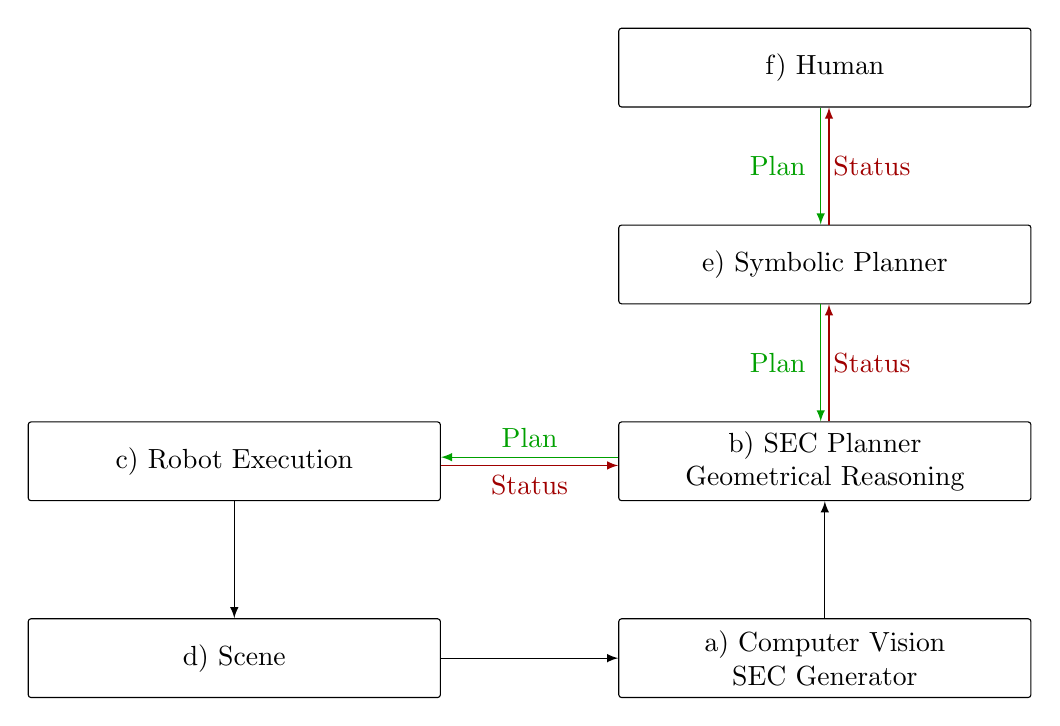
\begin{tikzpicture}[node distance=2.5cm, auto]
	\node [block] (scene) {d) Scene};
	\node [block, right of=scene, node distance=7.5cm] (computervision) {a) Computer Vision\\SEC Generator};
	\node [block, above of=computervision] (planner_sec) {b) SEC Planner\\Geometrical Reasoning};
	\node [block, above of=planner_sec] (planner_highlevel) {e) Symbolic Planner};
	\node [block, above of=planner_highlevel] (planner_human) {f) Human};
	\node [block, above of=scene] (robot) {c) Robot Execution};

	\draw [arrow] (robot.south) to (scene.north);
	\draw [arrow] (scene.east) to (computervision.west);
	\draw [arrow] (computervision.north) to (planner_sec.south);

	% Planner SEC
	\draw [arrow, color=green1] ([yshift=0.15em] planner_sec.west) to node[arrowtext, above, name=plan] {Plan} ([yshift=0.15em] robot.east);
	\draw [arrow, color=red1] ([yshift=-0.15em] robot.east) to node[arrowtext, below, name=error] {Status} ([yshift=-0.15em] planner_sec.west);

	% High level
	\draw [arrow, color=red1] ([xshift=0.15em] planner_sec.north) to node[arrowtext, right, name=error, xshift=-0.8em] {Status} ([xshift=0.15em] planner_highlevel.south);
	\draw [arrow, color=green1] ([xshift=-0.15em] planner_highlevel.south) to node[arrowtext, left, name=plan, xshift=0.8em] {Plan} ([xshift=-0.15em] planner_sec.north);

	% Human
	\draw [arrow, color=red1] ([xshift=0.15em] planner_highlevel.north) to node[arrowtext, right, name=error, xshift=-0.8em] {Status} ([xshift=0.15em] planner_human.south);
	\draw [arrow, color=green1] ([xshift=-0.15em] planner_human.south) to node[arrowtext, left, name=plan, xshift=0.8em] {Plan} ([xshift=-0.15em] planner_highlevel.north);
\end{tikzpicture}

  \caption{The structure resembles \figref{fig:sec_usingaffordanceforplanning_plannerstructure}, but includes e) a symbolic planner. This planner includes high level knowledge as object properties or functions of objects.}
  \label{fig:sec_usingaffordanceforplanning_plannerstructurewithhighlevel}
\end{figure}

The here shown planning approach is entirely data-driven and bottom up.
This means, it generalizes well, except for those actions, which require high level knowledge: Here a second planner is needed.
This enables robots to plan complex action sequences in unknown --- and possibly even unstructured --- environments.
Apart from knowledge about tools, \eg a knife for cutting, the approach is even agnostic of object functions, size, or shape.
The resulting planning system bridges the signal-to-symbol gap in a natural way and allows for rapid planning even in complex environments.
